\documentclass{article}
\usepackage{graphicx}
\usepackage{titlesec}
\usepackage{float}
\usepackage{fancyhdr}
\usepackage[english]{babel}
\usepackage[margin=2.2cm]{geometry}
\usepackage[utf8]{inputenc}
\usepackage[T1]{fontenc}
\usepackage{subcaption}

\graphicspath{{figures/}}

\titleformat*{\section}{\LARGE\bfseries}
\titleformat*{\subsection}{\large\bfseries}
\titleformat*{\subsubsection}{\small\bfseries}
 
\pagestyle{fancy}
\fancyhf{}
\rhead{Joachim Tapparel and Lennard Ludwig}
\lhead{Mini-project 1 : Classification, weight sharing and auxiliary losses}
\cfoot{\thepage}

\begin{document}
\thispagestyle{fancy}

\section{The architectures}

\subsection{Simple Architecture}

In this first simple architecture, we simply provide the network a tensor containing both images in two different channels and pass it through the convolutional part of the network. At the end of this part we reshape the tensor to a 1d tensor and pass it through two successive linear layers to make the decision. The figure \ref{fig:simple} shows an implementation of this principle using three convolutional layers. 

\begin{figure}[H]
\centering{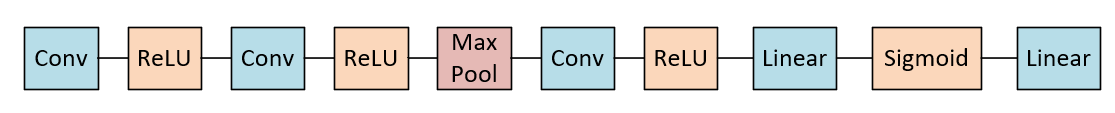
\includegraphics[width=0.6\textwidth]{arch_simple}}
\caption{Simple Architecture}
\label{fig:simple}
\end{figure}

In the beforehand scenario, the network doesn't take into account any information regarding the structure of the input, for example the fact that the input consists of two images containing numbers. This can be accounted for by using weight sharing as shown in the next part.

\subsection{Weight Sharing}

By using the structure of the input data, we can create two parallel paths to process each image separately and compare them afterwards. As both paths should train to recognize handwritten digits, it makes sense to share the weights between the two convolutional parts to achieve better performance. 

\begin{figure}[H]
\centering{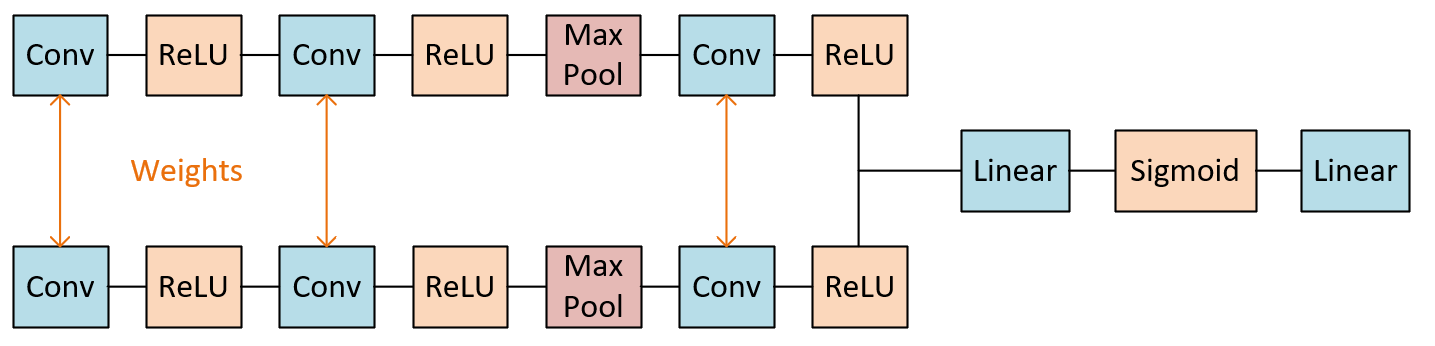
\includegraphics[width=0.6\textwidth]{arch_ws}}
\caption{Addition of weight sharing}
\end{figure}

After the convolutional part, we merge the two outputs together and make a decision. By doing this, we don't train the network to recognise the numbers them self, but only the combination of the images. This can be done using auxiliary losses. 

\subsection{Auxiliary losses}

The goal of auxiliary losses is to optimise some parts of the network to a specific task, in this case we can train the network to recognise numbers after the convolutional layers. Again we use weight sharing in those parts as they do the same job of recognising digits.

\begin{figure}[H]
\centering{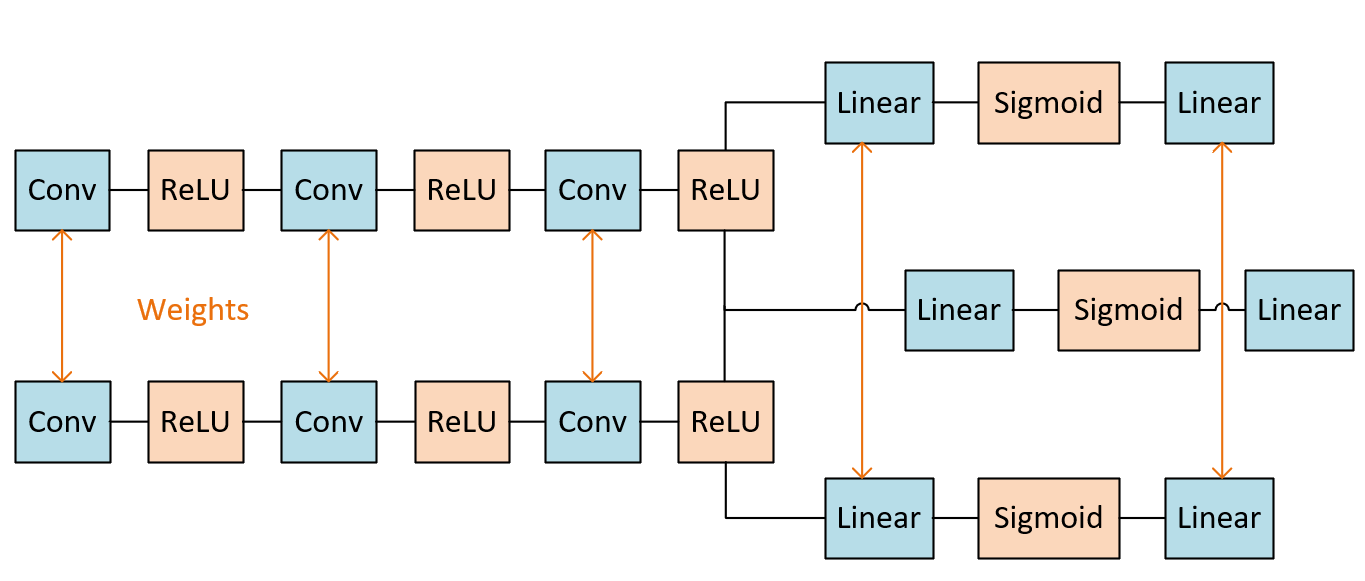
\includegraphics[width=0.6\textwidth]{arch_al}}
\caption{Addition of auxiliary losses}
\end{figure}

We expect this architecture to work better than the two previous ones as we use the information regarding the structure of the input data. 

\section{Results}

\subsection{Simple Architecture}
We tried different networks with one, two and three convolutional layers and keeping the number of parameters constant and there is no change in performance. By using the parameters and architecture in our code, with 25 epochs, a minibatch size of 50 and 1000 train samples, we get an error rate of 20.95\% with a standard deviation of 0.6241.

\subsection{Weight Sharing}

Again, the same way as before we tried different depths of convolutional layers, but this time we got better results by using three layers instead of one. Again, we kept the number of parameters constant.

\begin{center}
\begin{tabular}{|c|c|c|}
\hline 
\# of layers & \% of error & std deviation \\ 
\hline 
1 & 21.55 & 0.7382 \\ 
\hline 
2 & 18.62 & 0.8626 \\ 
\hline 
3 & 17.82 & 0.9028 \\ 
\hline 
\end{tabular}
\end{center} 

If we plot the output of the network in a plane (one hot output), we get the following graphs.

\begin{figure}[H]
\begin{center}
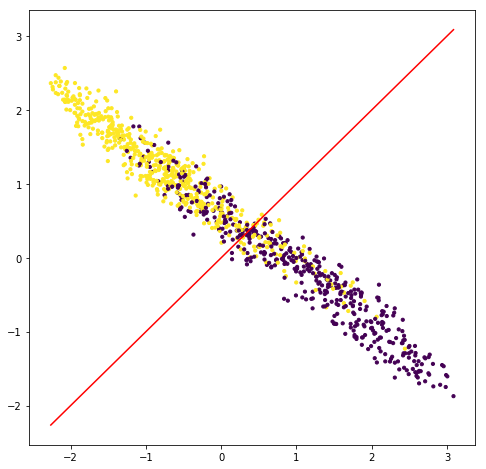
\includegraphics[width=0.25\textwidth]{ws_conv1}
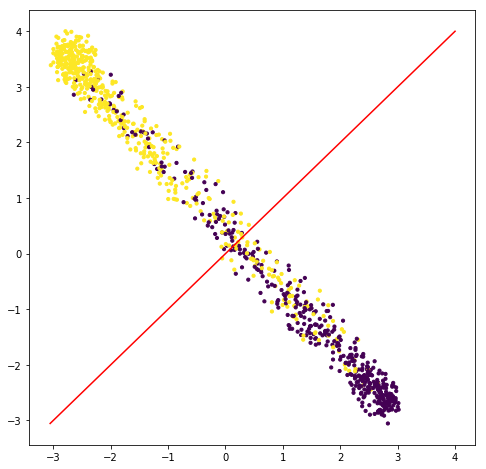
\includegraphics[width=0.25\textwidth]{ws_conv2}
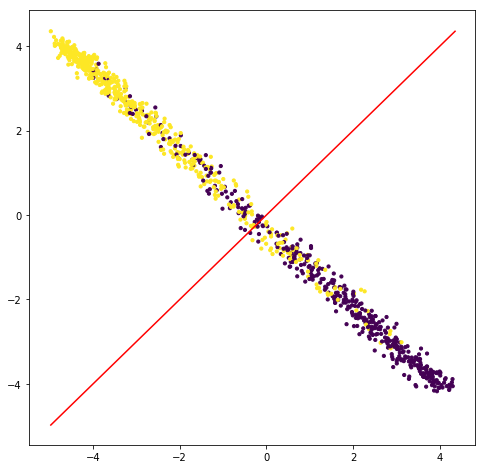
\includegraphics[width=0.25\textwidth]{ws_conv3}
\caption{Network output with one, two and three convolutional layer}
\end{center}
\end{figure}

In these graphs, the color of each point corresponds to the correct label and the red line is the decision boundary. In the ideal case fo a 100\% success rate we would have a yellow cluster on top and a purple cluster on the bottom. We can observe that with more layers, the output is spread further apart and thus tends to separate the clusters better.

\subsection{Auxiliary Losses}

As said before, with the auxiliary losses we expect the best results.

\begin{center}
\begin{tabular}{|c|c|c|}
\hline 
\# of layers & \% of error & std deviation \\ 
\hline 
1 & 26.85 & 3.35 \\ 
\hline 
2 & 14.62 & 0.9461 \\ 
\hline 
3 & 12.38 & 0.7208 \\ 
\hline 
\end{tabular}
\end{center}

And indeed we get the best results by using three convolutional layers, weight sharing and auxiliary losses with only 12.4\% of error. We can also notice that with only one layer, the result is worse than all of the tests above. This is due to the fact that the network isn't able to recognize the digits properly and thus influences the loss incorrectly.

\subsection{Comparison}

If we have a look at the plots of the outputs, we can observe that the further the network is able to spread the points, the better the performance. 

\begin{figure}[H]
\begin{center}
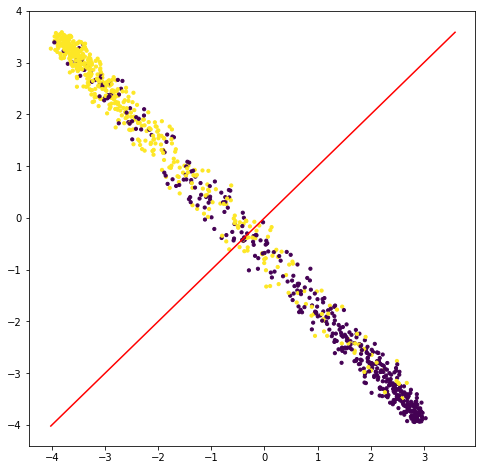
\includegraphics[width=0.25\textwidth]{simple_conv3}
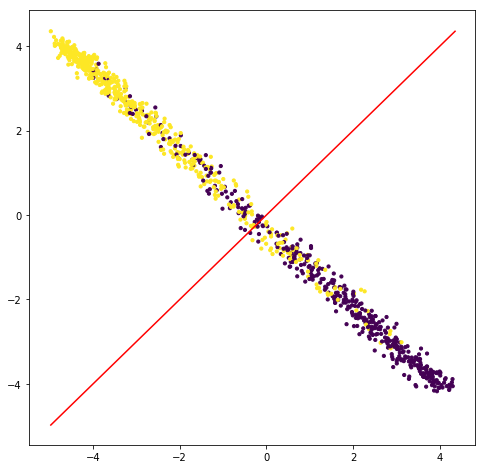
\includegraphics[width=0.25\textwidth]{ws_conv3}
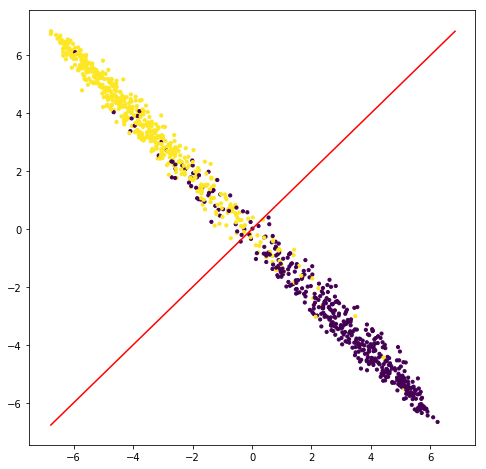
\includegraphics[width=0.25\textwidth]{al_conv3}
\caption{Network output with simple, weight sharing and auxiliary loss architecture with three convolutional layers each}
\end{center}
\end{figure}


\end{document}

%
%
%
%
%
%
%
%
%
%
%
%
%
%
%
%
%
%
%
%
%
%
%
%
%
%
%
